In this chapter, we analyze two proposed idealized models of the TCPC. These models are designed to incorporate key geometric modifications identified as beneficial in reducing energy dissipation, as described in \cite{Rijnberg2018}. These modifications, summarized in Figure~\ref{fig:positive_modifications}, serve as a foundation for investigating the effects of caval offsetting, curving, flaring, and other geometric factors on flow dynamics.

\begin{figure}[H]
	\centering
	\vspace{3mm}
	\includegraphics[width=0.65\textwidth]{figures/energyloss-en.pdf}
	\vspace{3mm}
	\caption[Positive Modifications for TCPC]{Key modifications to improve TCPC geometry and reduce energy dissipation: a) caval offsetting, where the inferior and superior vena cava are misaligned to minimize flow collision; b) curving, where the vessels are curved; c) the Y-graft configuration, which splits the flow evenly between outlets; and d) flaring, where the connections are widened to reduce sharp corners and flow resistance. Adapted from \cite{Rijnberg2018}.}
	\label{fig:positive_modifications}
\end{figure}

\section{The models}

To systematically evaluate the effects of geometric changes, the models were developed with varying levels of complexity, incorporating different numbers of degrees of freedom. Both models represent idealized TCPC geometries and share the same labeling convention for inlets and outlets. 

The inlets are denoted as $\Gamma^{\text{N}}_{\text{in}}$ (representing the superior vena cava at the top) and $\Gamma^{\text{S}}_{\text{in}}$ (representing the inferior vena cava with the conduit at the bottom). Similarly, the outlets are labeled as $\Gamma^{\text{W}}_{\text{out}}$ (representing the left part of the pulmonary artery) and $\Gamma^{\text{E}}_{\text{out}}$ (representing the right part of the pulmonary artery).
The shared geometric framework and boundary labels, is illustrated in Figure~\ref{fig:junction schema}. The dimensions of cylindrical segments forming the simplified junction are presented in Table~\ref{tab:tcpc dims}.


\begin{figure}[H]
	\centering
	\vspace{2mm}
	\includegraphics[width=0.99\textwidth]{figures/3d-tcpc-schema-combined.pdf}
	\vspace{7mm}
	\caption{Schematic representation of the idealized TCPC geometry. The labeled inlets ($\Gamma^{\text{N}}_{\text{in}}$, $\Gamma^{\text{S}}_{\text{in}}$) and outlets ($\Gamma^{\text{W}}{\text{out}}$, $\Gamma^{\text{E}}{\text{out}}$), directions of inflows and outflows, and the dimensions of the cylindrical segments forming the junction are illustrated.}
	\label{fig:junction schema}
\end{figure}

\bgroup
\centering
\vspace{2mm}
\setlength\tabcolsep{3mm}
\def\arraystretch{1.7}%
\begin{tabular}{|l|l|c|c|}
	\hline
	Segment & Abbreviation & Length & Diameter \\ \hline
	Inferior vena cava 	& IVC 	&      39 mm        &     14 mm    \\ 
	Superior vena cava  & SVC 	&      39 mm     	&     14 mm     \\ 
	Pulmonary artery 	& PA 	&      170 mm     	&     22 mm     \\  \hline
\end{tabular}
\vspace{2mm}
\captionof{table}{Dimensions of the cylindrical segments forming the idealized TCPC junction.}
\label{tab:tcpc dims}
\egroup

\subsection*{Model 1: Simplified cylindrical junction}

The first model represents a basic cylindrical junction, where the bottom vertical cylinder corresponds to the inferior vena cava (IVC), the horizontal cylinder corresponds to the pulmonary artery, and the top vertical cylinder represents the superior vena cava (SVC). The IVC and SVC are connected perpendicularly to the pulmonary artery, creating a cross-like structure. 

Model 1 was chosen because it introduces only one degree of freedom: the vertical offset of the IVC relative to the SVC. This simplicity makes it feasible to sample and evaluate the optimization space exhaustively, providing an opportunity to study the behavior of the objective functions, namely wall shear stress (WSS) and turbulence kinetic energy (TKE), in detail.

\subsection*{Model 2: More complex geometric model}
The second model introduces additional complexity by incorporating five degrees of freedom: the vertical offset of the IVC, the angles of connection for both the IVC and SVC to the pulmonary artery, the flaring of the IVC, and the width of the IVC. This model enables a more detailed investigation of the interaction between geometric parameters and hemodynamic efficiency.

Model 2 was selected because its higher complexity allows for greater variations in geometry and, consequently, a potentially larger impact on flow dynamics. However, the increased number of degrees of freedom makes it infeasible to sample the optimization space comprehensively, rendering the model more akin to a "black box" during optimization.

\begin{figure}[h]
	\begin{subfigure}{0.48\textwidth}
		\centering
		\includegraphics[width=0.91\textwidth, trim={0 0 0 0}]{figures/model1.pdf}
		\caption[Simplified Cylindrical Junction]{Schematic of Model 1: A simplified cylindrical junction with one degree of freedom, the vertical offset of the IVC relative to the SVC.}
		\label{fig:model1_schematic}
	\end{subfigure}\hfill%
	\begin{subfigure}{0.48\textwidth}
		\centering
		\includegraphics[width=0.91\textwidth]{figures/model2.pdf}
		\caption[Complex Geometric Model]{Schematic of Model 2: A more complex model with five degrees of freedom—IVC offset, connection angles, flaring, and width of the IVC.}
		\label{fig:model2_schematic}
	\end{subfigure}
\end{figure}
